\documentclass[../thesis.tex]{subfiles}
\begin{document}
\chapter{Experimental Results}
\label{ch:results}

\section{Overall Performance}

 \begin{figure}[H]
	\centering
	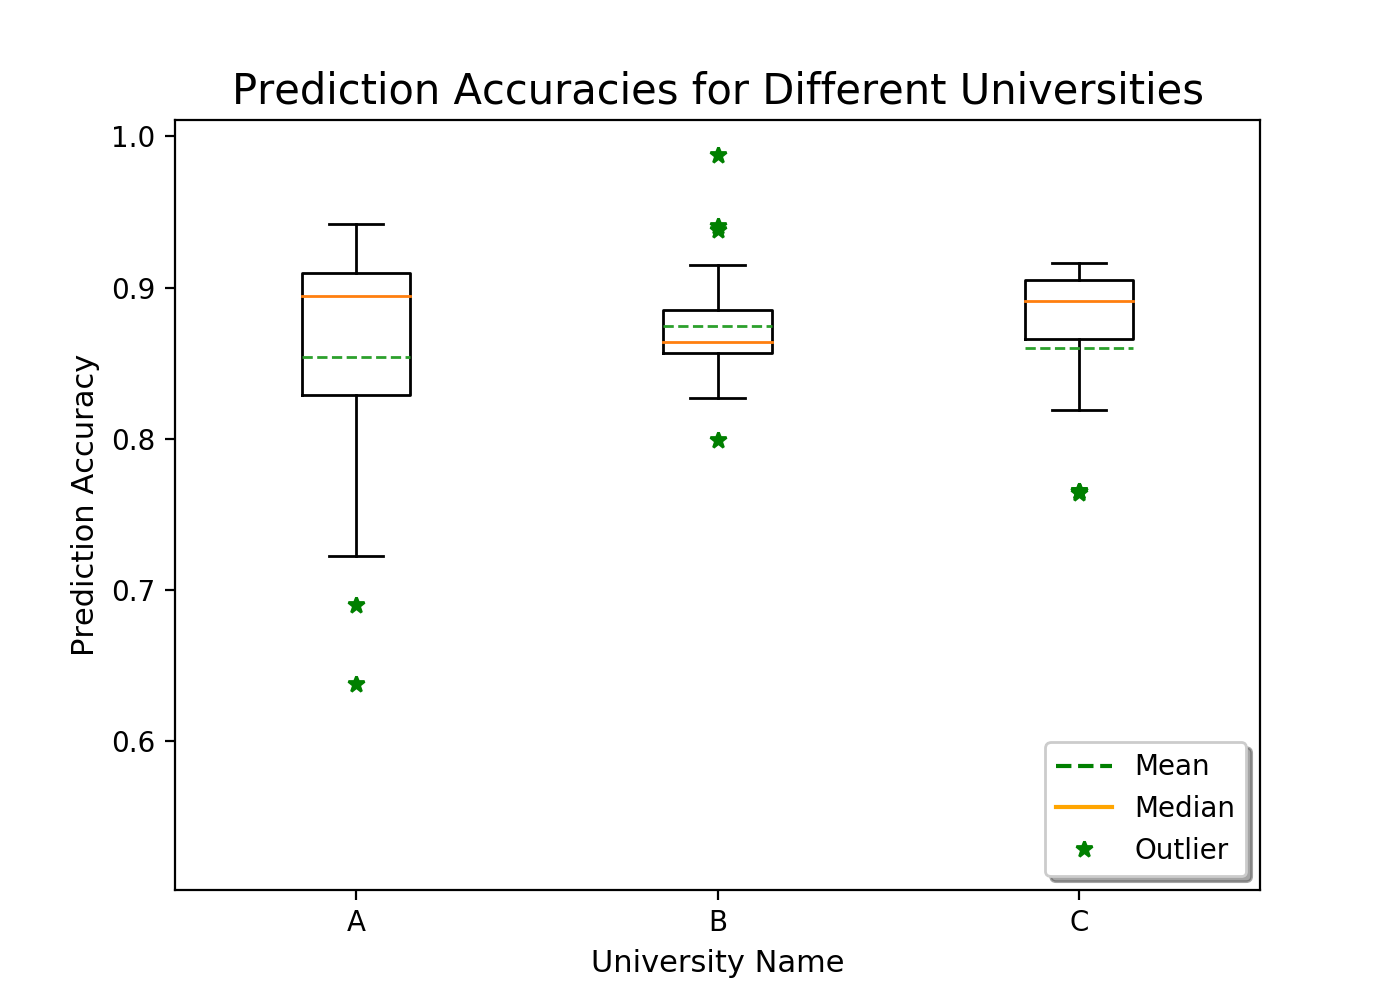
\includegraphics[width=\textwidth]{uni_analysis.png}
	\caption{Overall accuracy of the model for each set of university configurations used as the validation set.}
\end{figure}

In Figure 6.1, we show the overall accuracy of our model. For each university, we chose one snapshot in time and ran a LOO Cross Validation on all the device configurations. The the x-axis shows the name of the three anonymized universities used, and the y-axis shows prediction accuracies. The box plot is supposed to highlight the average (green dotted line), median (orange line) and upper ($Q_U$) and lower quartiles ($Q_L$). The box itself marks the Inter Quartile Range (IQR). The outliers (green stars) are all the data points that lie outside $Q_L - 1.5*IQR$ and $Q_U+1.5*IQR$. Our results in Figure 6.1 are after preprocessing the data and we see accuracies as high as 95\%, and an average of 80\%. These results are very promising as we see high accuracies using a fairly unmodified preexisting NLP algorithm. We next analyze how modifications to the model and to the training data affect our accuracies.

\section{Placeholders}

Generally, we see our accuracies increase when placeholders are used to substitute certain parameters. For each analysis, we took monthly snapshots of University A and replaced all the keywords associated with the particular placeholder being tested. We performed one reference test which did not use any placeholders and used that as a baseline for our accuracy. For example, in the reference test our model will try to predict the exact IP address (e.g. 192.168.1.1) while in the IP Address placeholder test, the model will simply suggest a generic IPADDRESS token.

\begin{figure}[H]
	\centering
	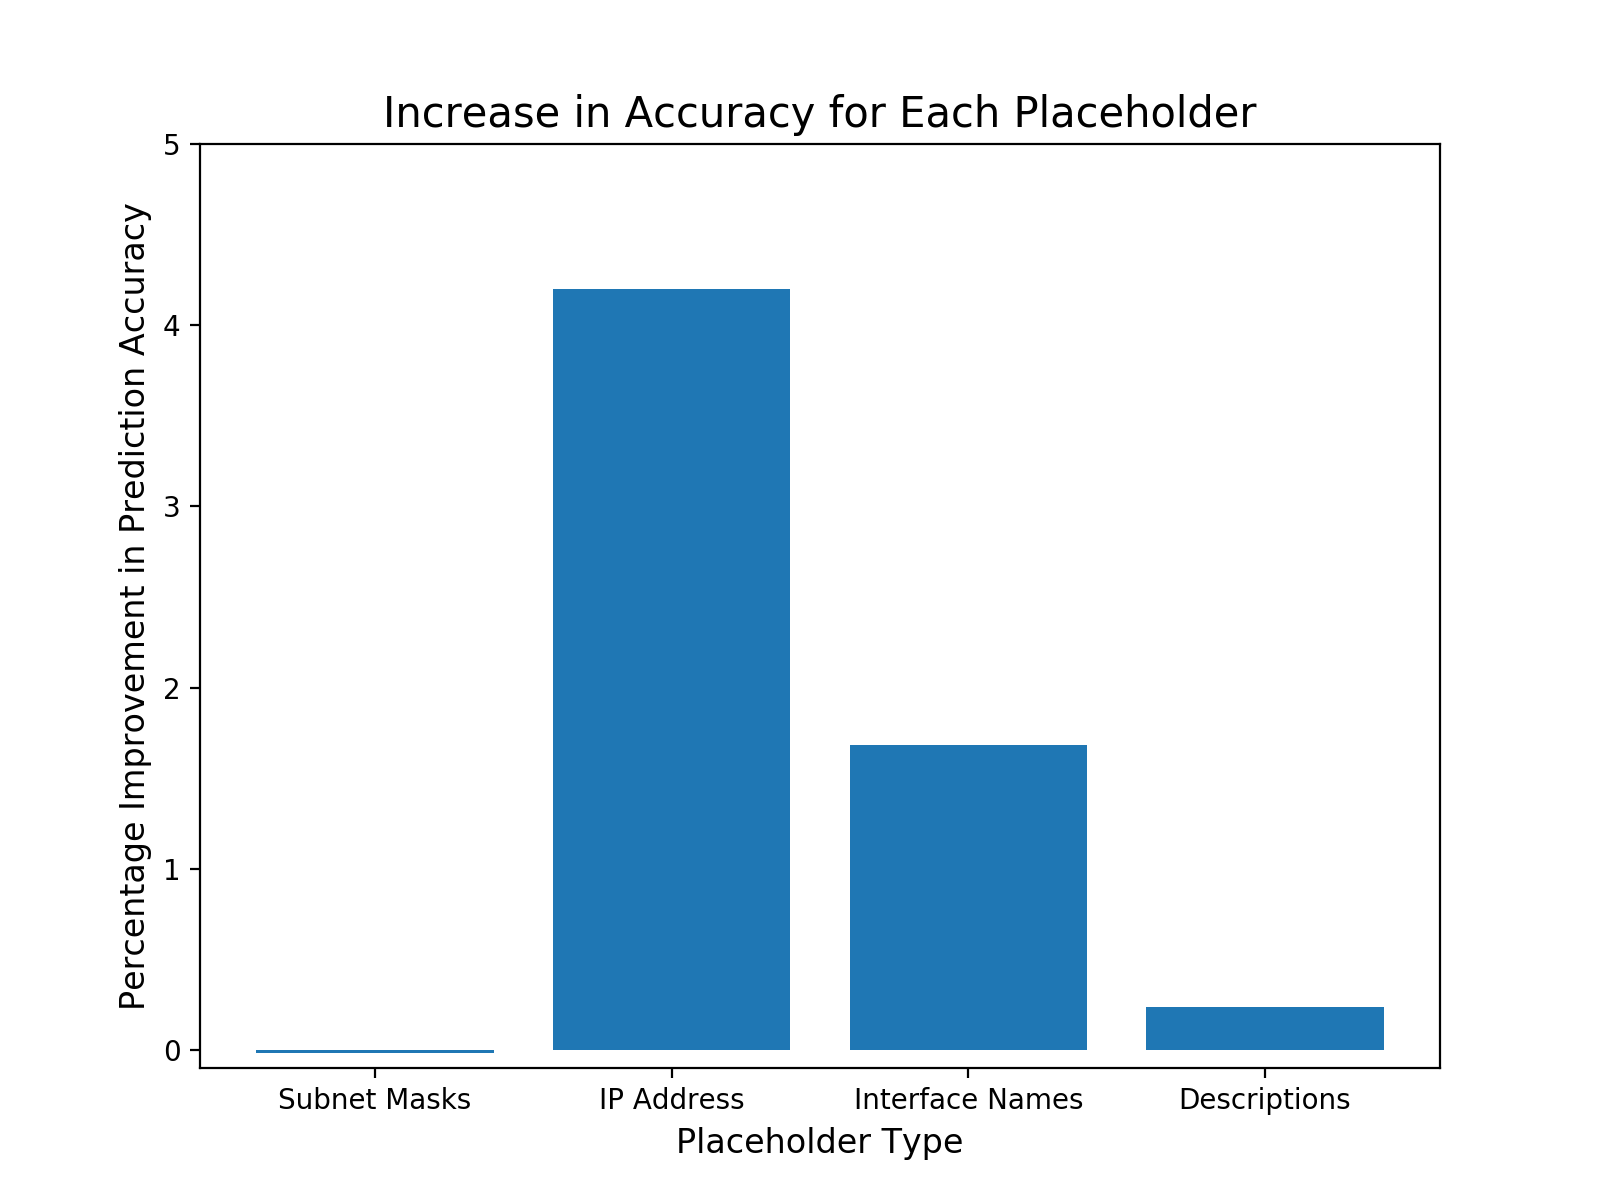
\includegraphics[width=\textwidth]{placeholders.png}
	\caption{Effect on Accuracy by Every Placeholder}
\end{figure}

As Figure 6.2 shows, the biggest jump in accuracy is accomplished by using IP address placeholders. This is expected, as configurations are bound to consist of a number of unique IP addresses which it makes it extremely difficult to predict which one is going to be used. Other tokens, for example subnet masks, tend to be much more homogeneous (usually a handful of subnet masks are repeatedly used across a network). Thus, we see an almost negligible improvement when replacing subnets. As placeholders were resulting in diminishing returns, we decided to go ahead with the ones we had implemented. We leave additional replacements (such as placeholders for VLAN names and routing costs) as a possible future extension.

\section{Length of Histories}

\begin{figure}[H]
	\centering
	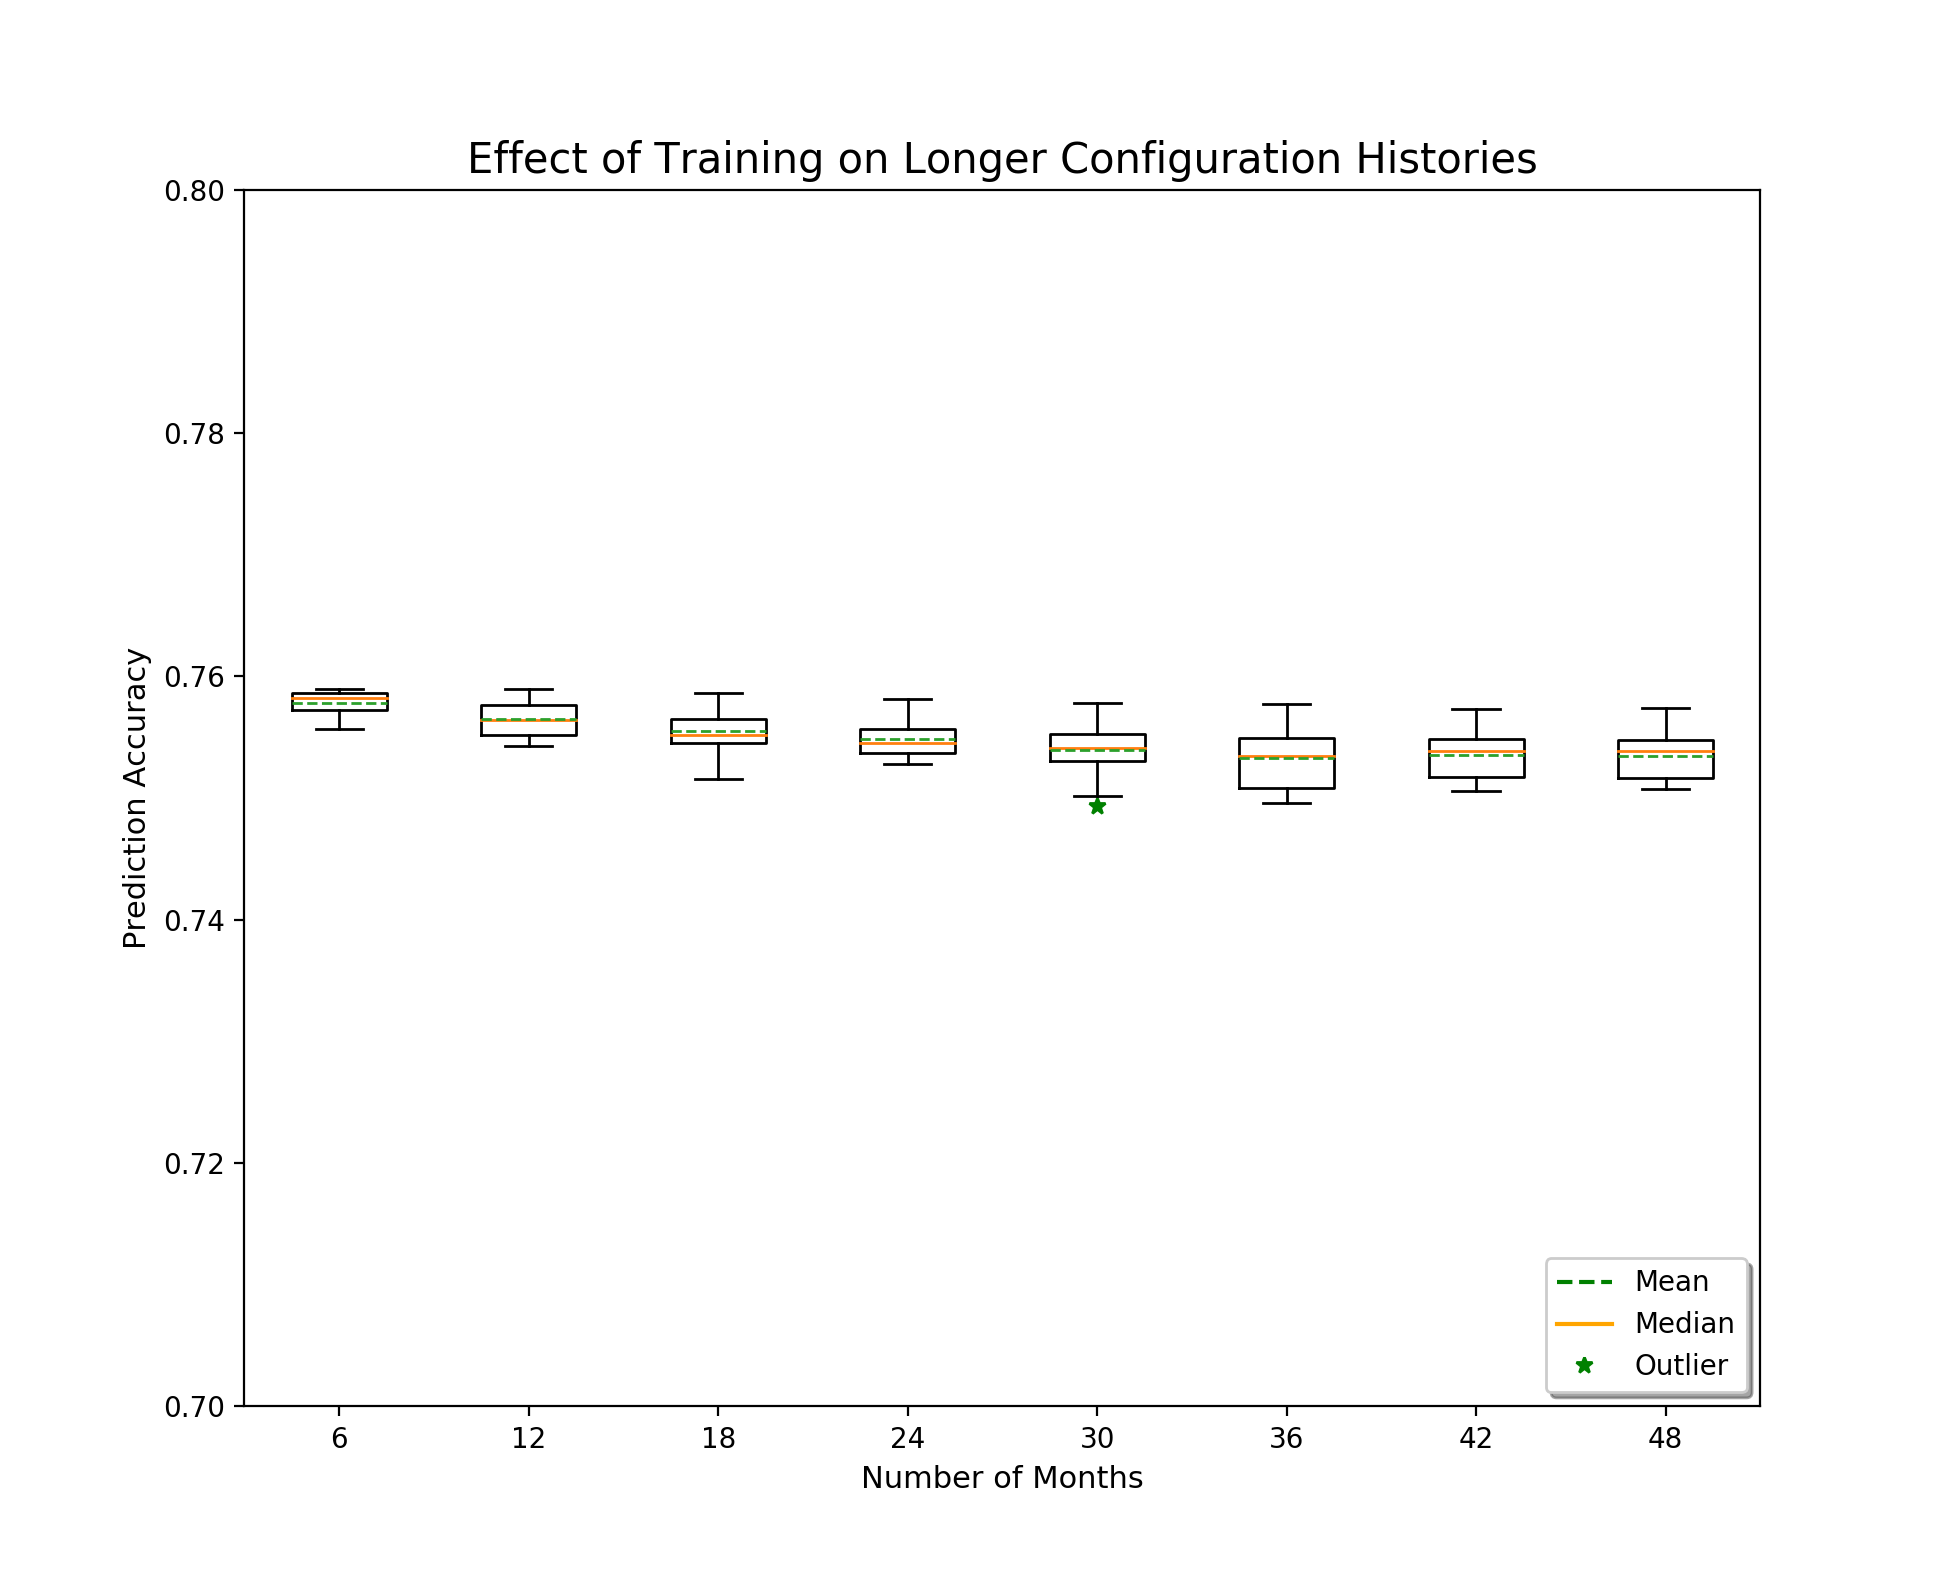
\includegraphics[width=\textwidth]{time.png}
	\caption{Longer histories may not result in higher accuracies.}
\end{figure}

As we had extensive data from University A's version control system, we analyzed the effect of selecting configurations across time on prediction accuracies. In Figure 6.3, the x-axis of the graph shows the number of months we chose to train on. As is apparent from the graph, if we train on longer configuration histories our accuracies stay about the same. In fact, we see a slight decrease which may be attributed to the variation introduced by the increased data points. It is a possibility that we might be overfitting on the parts of the configurations that remain unchanged over time. In a future analysis, one way to remediate this discrepancy would be to train on just the diffs of the configurations.
We should note that we do expect some change in the configurations over time as the university networks evolve. However, these changes tend to be small and homogeneous as the analyses from ~\cite{Kim} inform us. Similarly, another study done by ~\cite{Gember} observed that in most networks (80\%) there were a small number of change events (no more than 10). Furthermore, the study reveals that most change events seen across networks are small: in about half of the networks, a change event affects only one or two devices (on average). Thus, informed by existing research and our own analyses, we can expect our model to perform accurately without needing to train on data across multiple years.

\section{Number of Devices}
\begin{figure}[H]
	\centering
	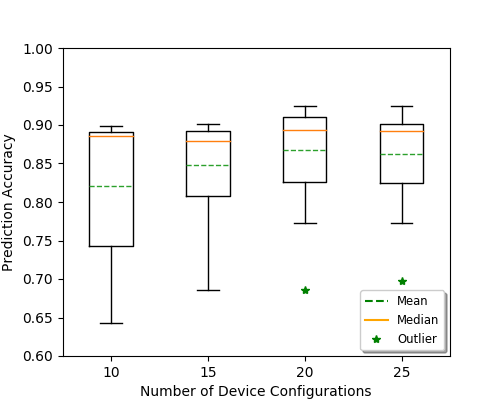
\includegraphics[width=\textwidth]{device_analysis.png}
	\caption{Training across more devices does improve accuracy to a certain point.}
\end{figure}

To obtain the results for Figure 6.4, we used configurations from University B and varied the number of devices to train on. We start by randomly selecting 10 devices for our initial training set. For each subsequent analysis, we continue randomly adding more devices to the existing training set. From the graph we can observe that as we add more device configurations, we see a slight increase in accuracy before it starts to give us diminishing returns. This may mean that the model has already seen most of the tokens that are often used by network operators. Every additional device contributes less to the overall model prediction set. In practice some devices being added may be different from the rest of the network, causing them to act as outliers which would be affecting our averages.

\section{Role-Based}

\begin{figure}[H]
	\centering
	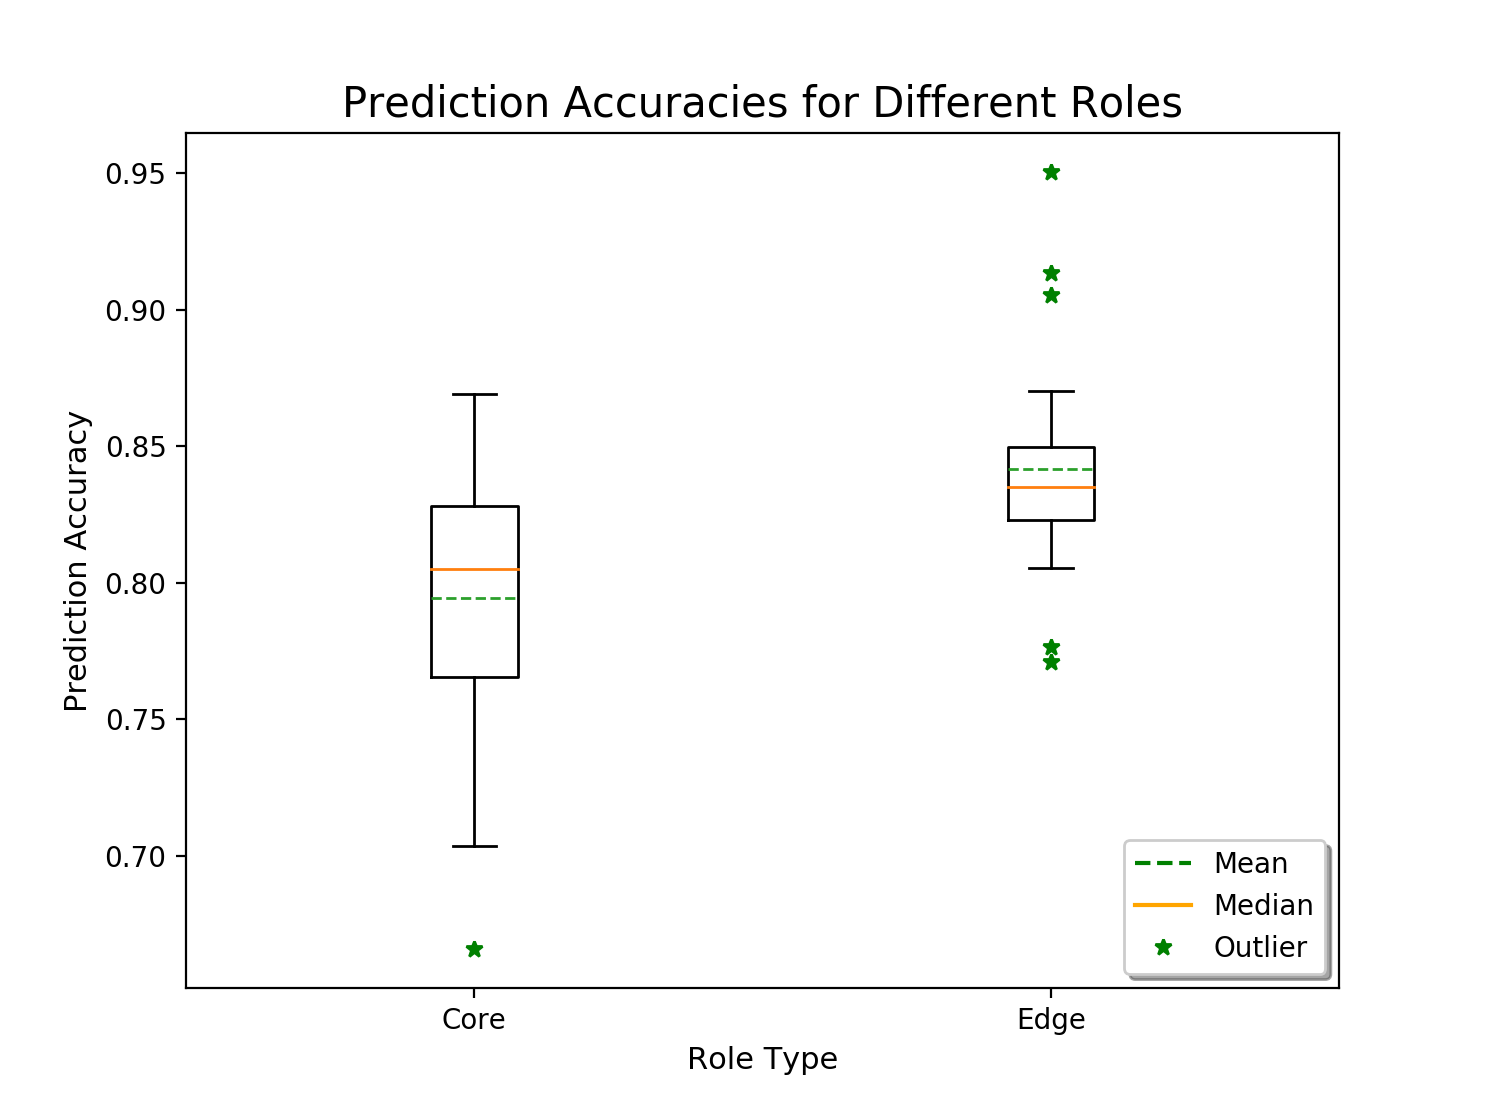
\includegraphics[width=\textwidth]{roles.png}
	\caption{Accuracies of models were trained on core and edge routers only, with the first boxplot showing the combined training set}
\end{figure}
In Figure 6.5, we analyse the effects of splitting the devices by their roles (explained in Section 1.3) and training the model on each role. We used data from University C as the router configurations were clearly labeled "edge" and "core". From the graph, we observe that splitting by roles did not result in an improvement in accuracy like we expected. There are a few factors that could be contributing to this result. It might be possible that there is not much variation in the two roles to begin with. We were assuming that the suggestions generated by the "combined" version would contain the tokens for both edge routers and core routers which would reduce the chances of the correct one cropping up in the top 3 suggested tokens. However, the results show that after separation, edge routers did not fare any better and core routers actually did worse. We also believe that this may be a problem of the labels/roles being coarsely defined as we were relying on the names of the routers to separate them. It is entirely possible that network operators may be labeling the routers as a rough approximation of their intended roles. Thus researchers may need to figure out a more fine grained way about dividing them.\\

\section{Key Observations}
Our analyses show that the model performs fairly accurately after some preprocessing to the data in the form of placeholders. We can see that it is reasonably resilient to data scarcity across time and length, though we acknowledge that the homogeneity of the networking configurations may be a contributing factor to this observation. Finally, our analysis of router roles gives us an unexpected result. We believe further analyses on the contents of the configurations pertaining to different roles could help determine whether separation by roles is justified.

\end{document}
